%%%%%%%%%%%%%%%%%%%%%%% file template.tex %%%%%%%%%%%%%%%%%%%%%%%%%
%
% This is a general template file for the LaTeX package SVJour3
% for Springer journals.          Springer Heidelberg 2010/09/16
%
% Copy it to a new file with a new name and use it as the basis
% for your article. Delete % signs as needed.
%
% This template includes a few options for different layouts and
% content for various journals. Please consult a previous issue of
% your journal as needed.
%
%%%%%%%%%%%%%%%%%%%%%%%%%%%%%%%%%%%%%%%%%%%%%%%%%%%%%%%%%%%%%%%%%%%
%
% First comes an example EPS file -- just ignore it and
% proceed on the \documentclass line
% your LaTeX will extract the file if required

\RequirePackage{fix-cm}
%
%\documentclass{svjour3}                     % onecolumn (standard format)
%\documentclass[smallcondensed]{svjour3}     % onecolumn (ditto)
%\documentclass[smallextended]{svjour3}       % onecolumn (second format)
\documentclass[twocolumn]{svjour3}          % twocolumn
%
\smartqed  % flush right qed marks, e.g. at end of proof
%
\usepackage{graphicx}
\usepackage{amssymb}
\usepackage[ruled,vlined]{algorithm2e}
\usepackage{url}
\usepackage{hyperref}
%
% \usepackage{mathptmx}      % use Times fonts if available on your TeX system
%
% insert here the call for the packages your document requires
%\usepackage{latexsym}
% etc.
%
% please place your own definitions here and don't use \def but
% \newcommand{}{}
%
% Insert the name of "your journal" with
\journalname{Food and Bioprocess Technology}
%
\begin{document}

\title{Vision-Based Potato Blemish Detection via Interactive Image Segmentation%\thanks{Grants or other notes
%about the article that should go on the front page should be
%placed here. General acknowledgments should be placed at the end of the article.}
}
%\subtitle{Do you have a subtitle?\\ If so, write it here}

%\titlerunning{Short form of title}        % if too long for running head

\author{Ran Song*         \and
        Hossein Malekmohamadi* \and
				Jamie Hutton \and
				Glyn Happer \and 
				Tom Duckett
}

%\authorrunning{Short form of author list} % if too long for running head

\institute{* denotes equal contribution to this paper.\\
\\
                Ran Song \at
              School of Computer Science, University of Lincoln, Lincoln, UK \\
              \email{sora1998@hotmail.com}           %  \\
           \and
           Hossein Malekmohamadi \at
             School of Computer Science, University of Lincoln, Lincoln, UK \\
						\email{hmalek@lincoln.ac.uk}  
						\and
						Jamie Hutton \at
						School of Computer Science, University of Lincoln, Lincoln, UK
						\and
						Glyn Happer \at
						AHDB Potato Council, Sutton Bridge Crop Storage Research, Spalding, UK\\
						\email{Glyn.Harper@potato.ahdb.org.uk}
						\and
						Tom Duckett\at
             School of Computer Science, University of Lincoln, Lincoln, UK \\
						\email{tduckett@lincoln.ac.uk}
}

\date{Received: date / Accepted: date}
% The correct dates will be entered by the editor


\maketitle

\begin{abstract}
We present a vision-based system for detecting potato blemishes. It is a feasible solution to quality control tasks mainly because it adopts a novel scheme of interactive image segmentation. In general, our system incorporates the interactive acquisition of vision-based training data into the automatic classification using adaptive boosting. To reduce the manual effort required for interactively collecting the online training data, the input images are efficiently processed through GPU-based over-segmentation. We also developed a user-friendly graphical user interface which allows users to edit (select, deselect and reselect) the training data. It also allows the users to add more training data to improve the classifier if necessary. In contrast to the state-of-the-art methods which typically rely on offline training using a large collection of data, our system relies only on a tiny amount of training data offered by the users in an interactive manner. The experiments demonstrate that our system efficiently and effectively detects potato blemishes and can be potentially used for some other food processing applications.  
\keywords{Potato \and Interactive Image Segmentation \and Classification \and Adaboost \and Over-segmentation}
% \PACS{PACS code1 \and PACS code2 \and more}
% \subclass{MSC code1 \and MSC code2 \and more}
\end{abstract}

\section{Introduction}
\label{sec:intro}
It has been more than two decades since computer vision techniques were applied to automatic inspection of food products for quality assurance \cite{DE90}. The essential motivation is to use such techniques to replace or argument human inspectors for the evaluation of a variety of quality attributes of raw and prepared foods \cite{SG96}. Benefiting from the rapid development of commercial computing and sensing technologies, computer vision systems designed for food quality assurance have been able to provide a high level of flexibility and repeatability at relatively low cost. In sharp contrast, labour cost has been widely increased in the food industry where manufactures typically have a low profit margin. Also, consumers tend to buy the food products which look good since in most cases, it is not possible to directly taste the food (e.g., potato) when buying it. Hence, many companies in the food industry are willing to invest in proper computer vision techniques to reduce the cost as well as to boost sales. 

Potato is one of the most important foods in human history and currently accounts for $70-80\%$ of the carbohydrate consumed in the UK. The development of a vision-based system for detecting potato blemishes is not just economically significant, but also has a great potential to benefit quality assurance for other types of food due to the high visual variation of potatoes. This paper presents a prototype system for detecting potato blemishes using state-of-the-art computer vision techniques. It is composed of a computer and a light box  as shown in Fig.~\ref{fig:pro} where a digital SLR camera is fixed inside. The novelty of the proposed system is summarised as below:

\begin{enumerate}
\item The system relies merely on a tiny amount of training data in comparison with existing methods.
\item It enables a quantitative evaluation and analysis for the quality control of potatoes which is unavailable under the current working mode in industry.
\item The system is much more efficient than existing methods mainly due to the GPU-based implementation and the novel image processing pipeline based on classification of superpixels rather than pixels.
\item To the best of our knowledge, for the first time, a manual `correction mechanism' is incorporated into a vision-based system designed for the quality control of potatoes. This is achieved by the novel interactive training which essentially is a human-in-the-loop scheme. 
\end{enumerate}

\begin{figure}[t]
\centering
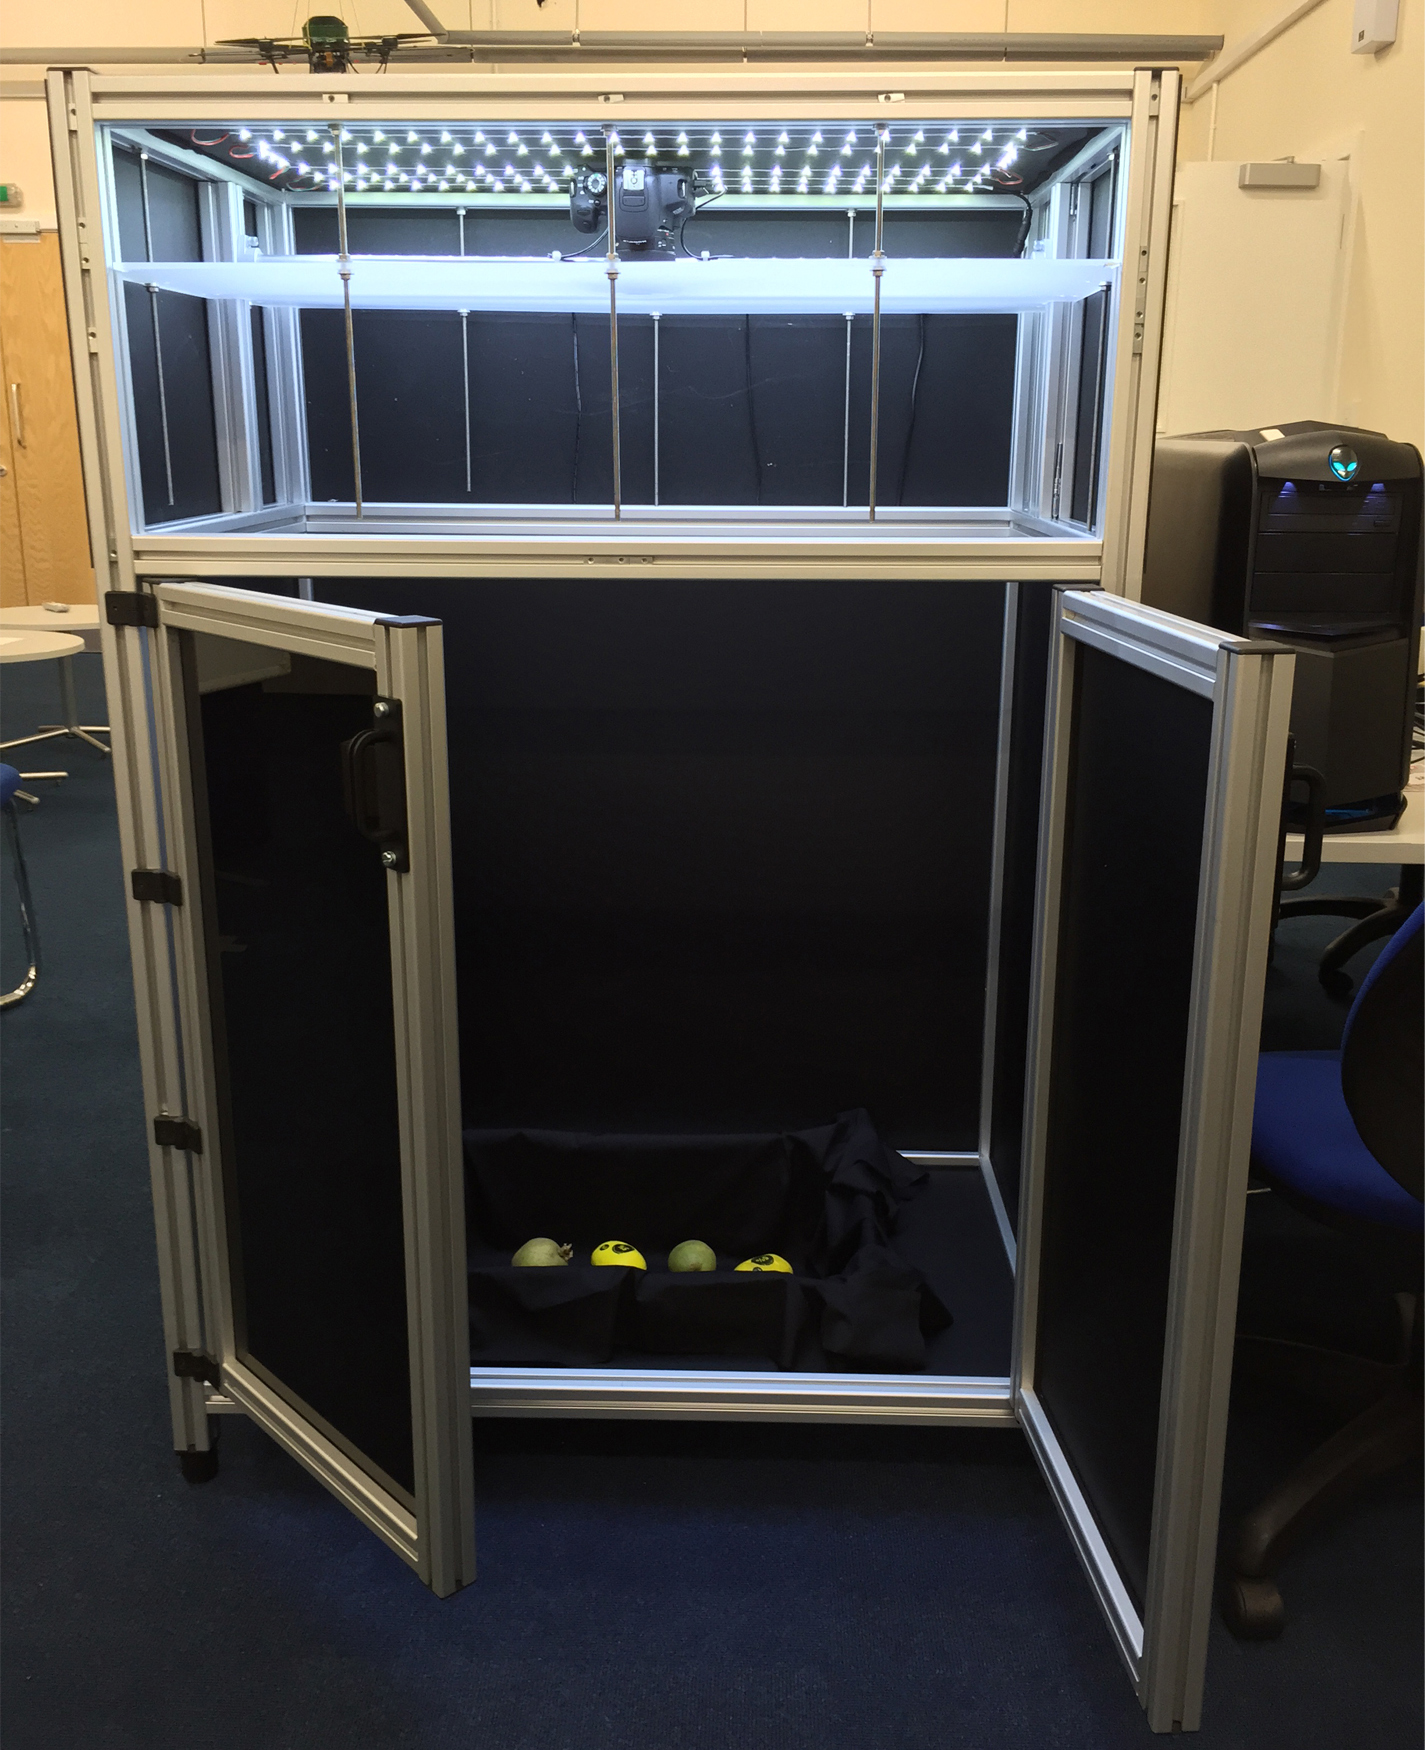
\includegraphics[width=0.95\linewidth]{lightbox.jpg}
\caption{The light box of the proposed prototype system for vision-based potato blemish detection It can be seen that a digital SLR camera is fixed at the top of the light box and connected with the computer next to it. To reduce reflection, we laid the array of LED lights in a diffusion box where its front panel has been taken out.}
\label{fig:pro}
\end{figure}

\subsection{Related work}
Barni \textit{et al.} \cite{BM97} presented an intelligent vision-based system for detecting defects on chicken meat. Defects were detected based on the analysis of the chromatic content of chicken images. Possible defect areas were first extracted by means of morphological image reconstruction and then classified according to a predefined list of defects. Russo \textit{et al.} \cite{RR02} a system for monitoring the production of fast food using a single static camera. By analysing the video with some computer vision techniques, a description of the fast food is produced for the ingredients and their physical arrangement to make sure that the food was produced correctly. Lee \textit{et al.} \cite{LK07} used colour information for monitoring food processing applications involving live products and biomaterials. Their system detected features based on colours and then employed principal component analysis to characterise target features from a set of training data. More recently, Joutou \textit{et al.} \cite{JT09} also investigated colour features where the food image recognition system also used other types of features such as texture and Scale invariant Feature Transform (SIFT) \cite{LD04}. Then, the multiple kernel learning method was employed to estimate the optimal weights to combine these features for each category of food. Yang \textit{et al.} \cite{YS10} presented another food recognition system which utilised a novel representation for food items that calculates pairwise statistics between local features computed over a soft pixel-wise segmentation of the image into eight ingredient types. The classification was based on the multi-dimensional histogram of these statistics. Boiman and Irani \cite{BO07} proposed a method to detect irregularities for fruit inspection by comparing a test image to a reference image representing the `good' case (expected or normal patterns). It generalised from the reference images and analysed the test images to find regions with low composition likelihood, which were considered as defects. To detect multiple food items from one food image, Matsuda and Yanai \cite{MY12} proposed a method based on co-occurrence statistics and manifold ranking.
\begin{figure*}[t]
\centering
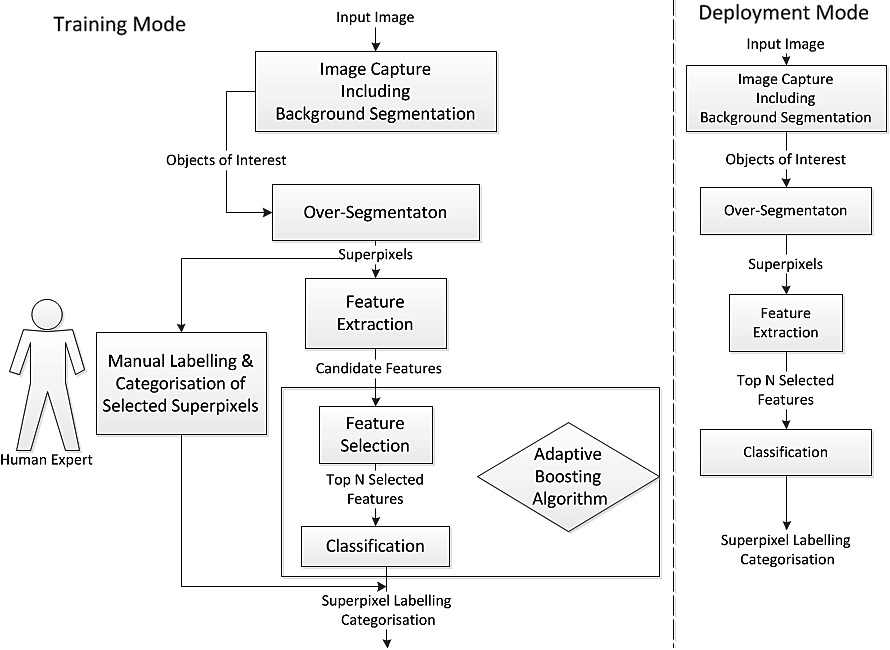
\includegraphics[width=0.9\linewidth]{overview.jpg}
\caption{Overview of our system}
\label{fig:ov}
\end{figure*} 

In particular, computer vision techniques have been used for inspecting potatoes for a long time. Tao \emph{et al.} \cite{TY95} used Fourier analysis to develop a classification method which achieved a high accuracy. Zhou \emph{et al.} \cite{ZL98} used green levels to detect greening and sprouting defects in potatoes. They also classified potatoes in terms of shape by comparison to an ellipse template, and in size and weight by measuring the minor axis and area, respectively. Recently, a method \cite{BM10} which used image segmentation algorithms to detect potatoes blemishes has been proposed. This method is based on training a pixel-wise classifier using features extracted from the image. However, the method is very slow although its classification achieves a high success rate. 

Many other related works where computer vision technology is used for food quality inspection can be found in the review papers \cite{GS96,BT04,ZC06,WD13,JP13}. 

\subsection{Our system}
It can be seen that there are several common issues existing in the vision-based techniques for food quality inspection. 

Firstly, the efficiency of the technique is vital since food products are typically fast-moving consumer goods. It is common that a huge amount of food products (e.g., potatoes) need to be handled every day in food processing and packaging factories. 

Secondly, due to the variety and the variation of food, most of the systems require a large dataset for training purpose in order to cover each type of defects, which could be extremely occasional, but do exist. However, it is not always easy to collect sufficient data for training because a food product could change rapidly in terms of colour, intensity, shape and volume, and these features are important in most of the aforementioned techniques. Typically, such a data collection could take a couple of months (e.g., the Supermarket Produce dataset was the result of 5 months of on-site collecting in a local fruit and vegetable distribution centre \cite{RA10}).

Thirdly, since usually a food company does not only process one type of food product (especially if the food is seasonal), the systems need to be periodically retrained to adapt to different food products. This means that the time-consuming offline training, as well as the extra effort needed to prepare the new training data (e.g., manually labelling the images of another product) could be very inconvenient for practical applications.

Finally and most importantly, to the best of our knowledge, there is no manual `correction mechanism' involved in any of the existing vision-based systems for food quality assurance. This is a waste of the expertise of the very people using the systems. They are typically quality control inspectors who possess a significant amount of knowledge about the possible defects. Moreover, safety standards on food products are quite strict since a bad product could cause serious troubles and the producer might face huge fines and compensations. Therefore, from a practical point of view, it is very important to introduce some manual correction mechanism as there is no guarantee that the automatic system can always deliver successful quality inspection. When the automatic system cannot recognise a certain defect, the human inspector should be allowed to step in and offer the particular help to the system to correct the error. 

These four issues form the motivation of developing our novel system designed specifically for detecting potato blemishes but with potential application to many other food products besides (e.g., fruits, beans, etc.). Fig.~\ref{fig:pro} shows the hardware components of the prototype system. With regard to the software, its most novel component is the idea of using real-time interactive image segmentation. To realise this idea, we develop a novel mechanism to help users to conveniently select the training data that they think necessary in an interactive manner. An adaptive boosting (AdaBoost) classifier \cite{SR99} which enables feature selection is then trained using the manually selected data. And the test image can be assessed by the trained classifier in real-time since only the selected features need to be calculated during the classification. In the next section, we give the technical details of the user-friendly mechanism which enables the interactive training, as well as the classification based on a set of image features selected using AdaBoost. 

\section{Interactive image classification via Adaboost classification}
Normally, to train the classifiers and test their performance, the images are marked up by hand to provide the ground truth information indicating the correct class of each pixel. Most existing publicly available databases which benchmark image segmentation techniques work in this way. However, due to the variety of visual appearance of potatoes, it is not realistic to apply such a strategy to the real tasks of potato quality inspection. Note that one specificity of potato is that its appearance changes rapidly and significantly over time and in many cases, time is the very reason that some defects occur. This is quite different from the objects in the image databases (e.g., the MSRC image database\footnote{\url{http://research.microsoft.com/en-us/projects/objectclassrecognition/}}) for benchmarking general image segmentation or object classification methods where the objects are generally invariant within a certain period of time. Such a specificity makes the conventional offline training based on a large set of previously constructed ground truth data unreliable. This is why it is so important to implement the online training using the currently available data. To achieve this, we developed the system illustrated in Fig.~\ref{fig:ov}. 
\begin{figure}[t]
\centering
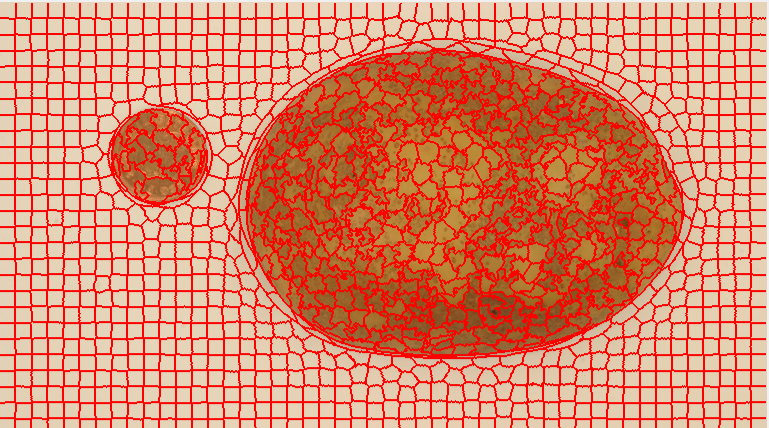
\includegraphics[width=1\linewidth]{superpixel.jpg}
\caption{Visualisation of the over-segmentation for an image containing a coin and a potato using SLIC.}
\label{fig:sp}
\end{figure} 

In Fig.~\ref{fig:ov}, the training mode is designed for iteratively teaching the adaptive boosting algorithm to distinguish between different categories. This stage requires the user to select and label a set of blemishes, which is used later for training the system. The user is then able to receive feedback by visually inspecting the accuracy of the classification. If mistakes are being made the user simply retrains the system. Once trained the system can be used in deployment mode, which means no more training is required to classify and diagnose blemishes. The user is able to swap back to training mode at any time to retrain after any classification mistakes. This procedure means there is no limitation on how many times the system can be trained, relying on experts to teach and guide the machine learning algorithm.

\subsection{Background segmentation}
The proposed system use a simple thresholding method for background segmentation. After the background segmentation, the user is not allowed to select any region in the background as the training data.
\subsection{Over-segmentation}
Image over-segmentation is used in our system to enhance the interactive mark-up. The process involves over-segmenting the captured image into local clusters (i.e., superpixels) which follow the contour of edges by colour or intensity differences. This approach aims to reduce redundancy in the image. Superpixels also allow an expert to select a relatively large area with only a single mouse click, which significantly mitigates the manual effort needed in the interactive scheme and makes it much more efficient. We employed the SLIC algorithm \cite{AR12} for over-segmentation where to further improve the efficiency, we apply the GPU version of SLIC \cite{RY11} in our system. It works by loading the cluster's information into local shared memory. In each iteration, after all pixels have been assigned a label, one thread per cluster is used to update the centres. As an example, the result of image over-segmentation is shown in Fig.~\ref{fig:sp}.

\subsection{Feature extraction}
In our system, a large collection of candidate features are required for each superpixel, from which the AdaBoost algorithm can select to build the classifiers. As suggested by \cite{BM10}, we use 7 colour channels: raw RGB, normalised RGB and the intensity channel. In \cite{BM10}, the image regions used for feature extraction were squares of size $33\times33, 65\times65, 97\times97, 129\times129$ and $161\times161$ pixels. Our system differs by using only superpixel regions, classifying each cluster of pixels based on their region characteristics. Superpixels reduce computation requirements in two aspects. Firstly, an image sized $1280\times720$ is represented as around $9200$ clusters requiring only $1\%$ of the computational resources when compared to pixel-wise classification. Secondly, the superpixel regions adapt to cluster together similar pixels, compensating for the requirement of using multiple region sizes.

We then consider the first three statistical moments for each superpixel: average (Eq.~(\ref{eq:av})), variance (Eq.~(\ref{eq:va})) and skewness (Eq.~(\ref{eq:sk})). 
\begin{equation}
\overline{x}=\frac{1}{N}\sum_{N}^{j=1}x_j;
\label{eq:av}
\end{equation}
\begin{equation}
Var(x_1 \ldots x_N)=\frac{1}{N-1}\sum_{N}^{j=1}(x_j-\overline{x});
\label{eq:va}
\end{equation}	
\begin{equation}
Skew(x_1 \ldots x_N)=\frac{1}{N}\sum_{N}^{j=1}(\frac{x_j-\overline{x}}{\sqrt{Var(x_1 \ldots x_N)}})^3.
\label{eq:sk}
\end{equation}

The first statistical moment is difficult to parallelize as this requires the implementation of a prefix-sum for the most optimal implementation, adding complexity with the use of shared memory. We use the large amount of segments produced by the gSLIC algorithm and sum each region on a separate thread using cluster centres. Once the first statistical movement has been calculated both variance and skewness are simple to implement. 

We calculate the three moments in each channel, resulting in 21 features. We also use a Sobel edge detector and a range filter in the intensity channel respectively. The aim of the edge detector is to determine the rate change in pixel intensities, which is a useful candidate feature for defects with a high rate of change. The range filter calculates the minimum, maximum and difference between the maximum and minimum values within a $5 \times 5$ neighbourhood. It indicates the roughness of a texture, aiding in the identification of defects. Then we compute the 3 moments on each of the resultant images, which produces 6 more features. We also record the longest Sobel edge length in each superpixel as a feature, which has been demonstrated experimentally useful for improving classification of some defects. Other features such as Gabor feature \cite{BM96} and Local Binary Features (LBP) \cite{OT02} were investigated experimentally as well. However, we found that they did not significantly improve the classification in our case while slowing down the processing. Finally, we incorporate 28 features in total into the classification. 
\begin{figure*} [t]
\centering
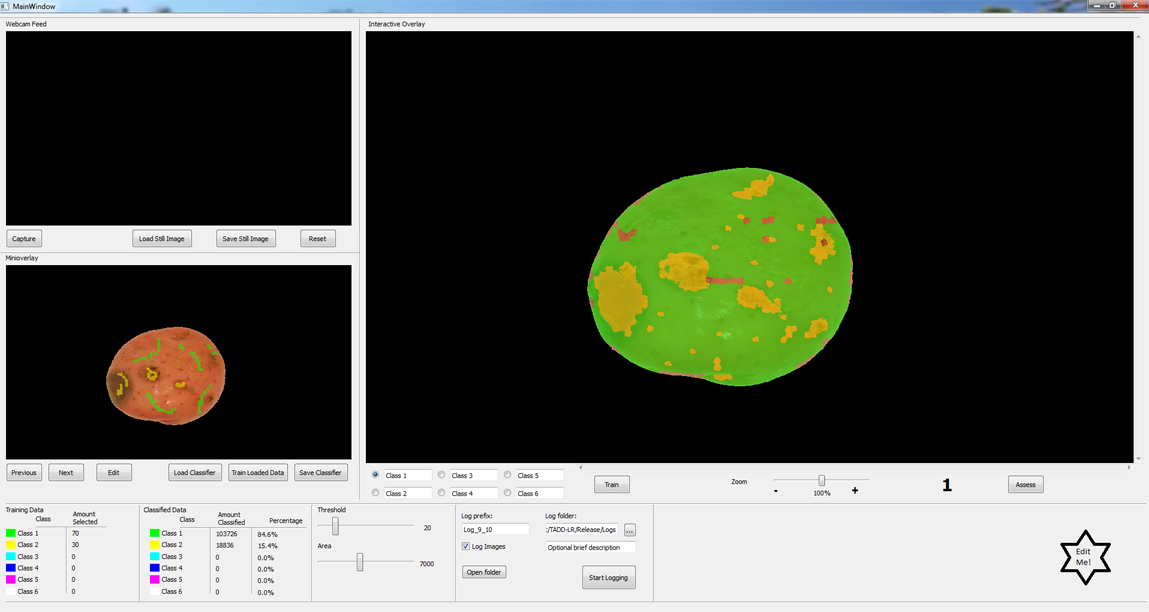
\includegraphics[width=0.96\linewidth]{gui.jpg}
\caption{The user-friendly GUI of the software}
\label{fig:gui}
\end{figure*}

\subsection{Classification via AdaBoost}
We employ the Adaptive Boosting (AdaBoost) algorithm proposed in \cite{BM10} to automatically select the best features for discriminating between defects and normal regions. The reason that we apply this algorithm in our system is that it can handle the natural variation in fresh produce due to different seasons and lighting conditions \cite{BM10}. Also, the method is able to build `minimalist' classifiers that optimise detection performance at low computational cost, which is very important for a real-time interactive system. 

This approach involves two stages: the first stage selects a feature set that will be used to train an AdaBoost classifier in the second stage. It also includes an additional step in order to limit the number of unique features used in the final classifier to a smaller number than the total number of weak classifiers allowed. 

We further developed a graphical user interface (GUI) as shown in Fig.~\ref{fig:gui}.  With such a GUI and the aforementioned techniques combined, our system allows users to select a handful of superpixels as the training data and the system can show the classification results based on the AdaBoost classifier trained by them in less than 1 second including visualisation. The users can then interactively improve the results by selecting new superpixels (or deselecting existing superpixels). We also upload a demonstration video to YouTube\footnote{\url{http://youtu.be/OXKyxHy4Vkg}} (1080p HD is available) to show how our system works.
\begin{figure*} [t]
\centering
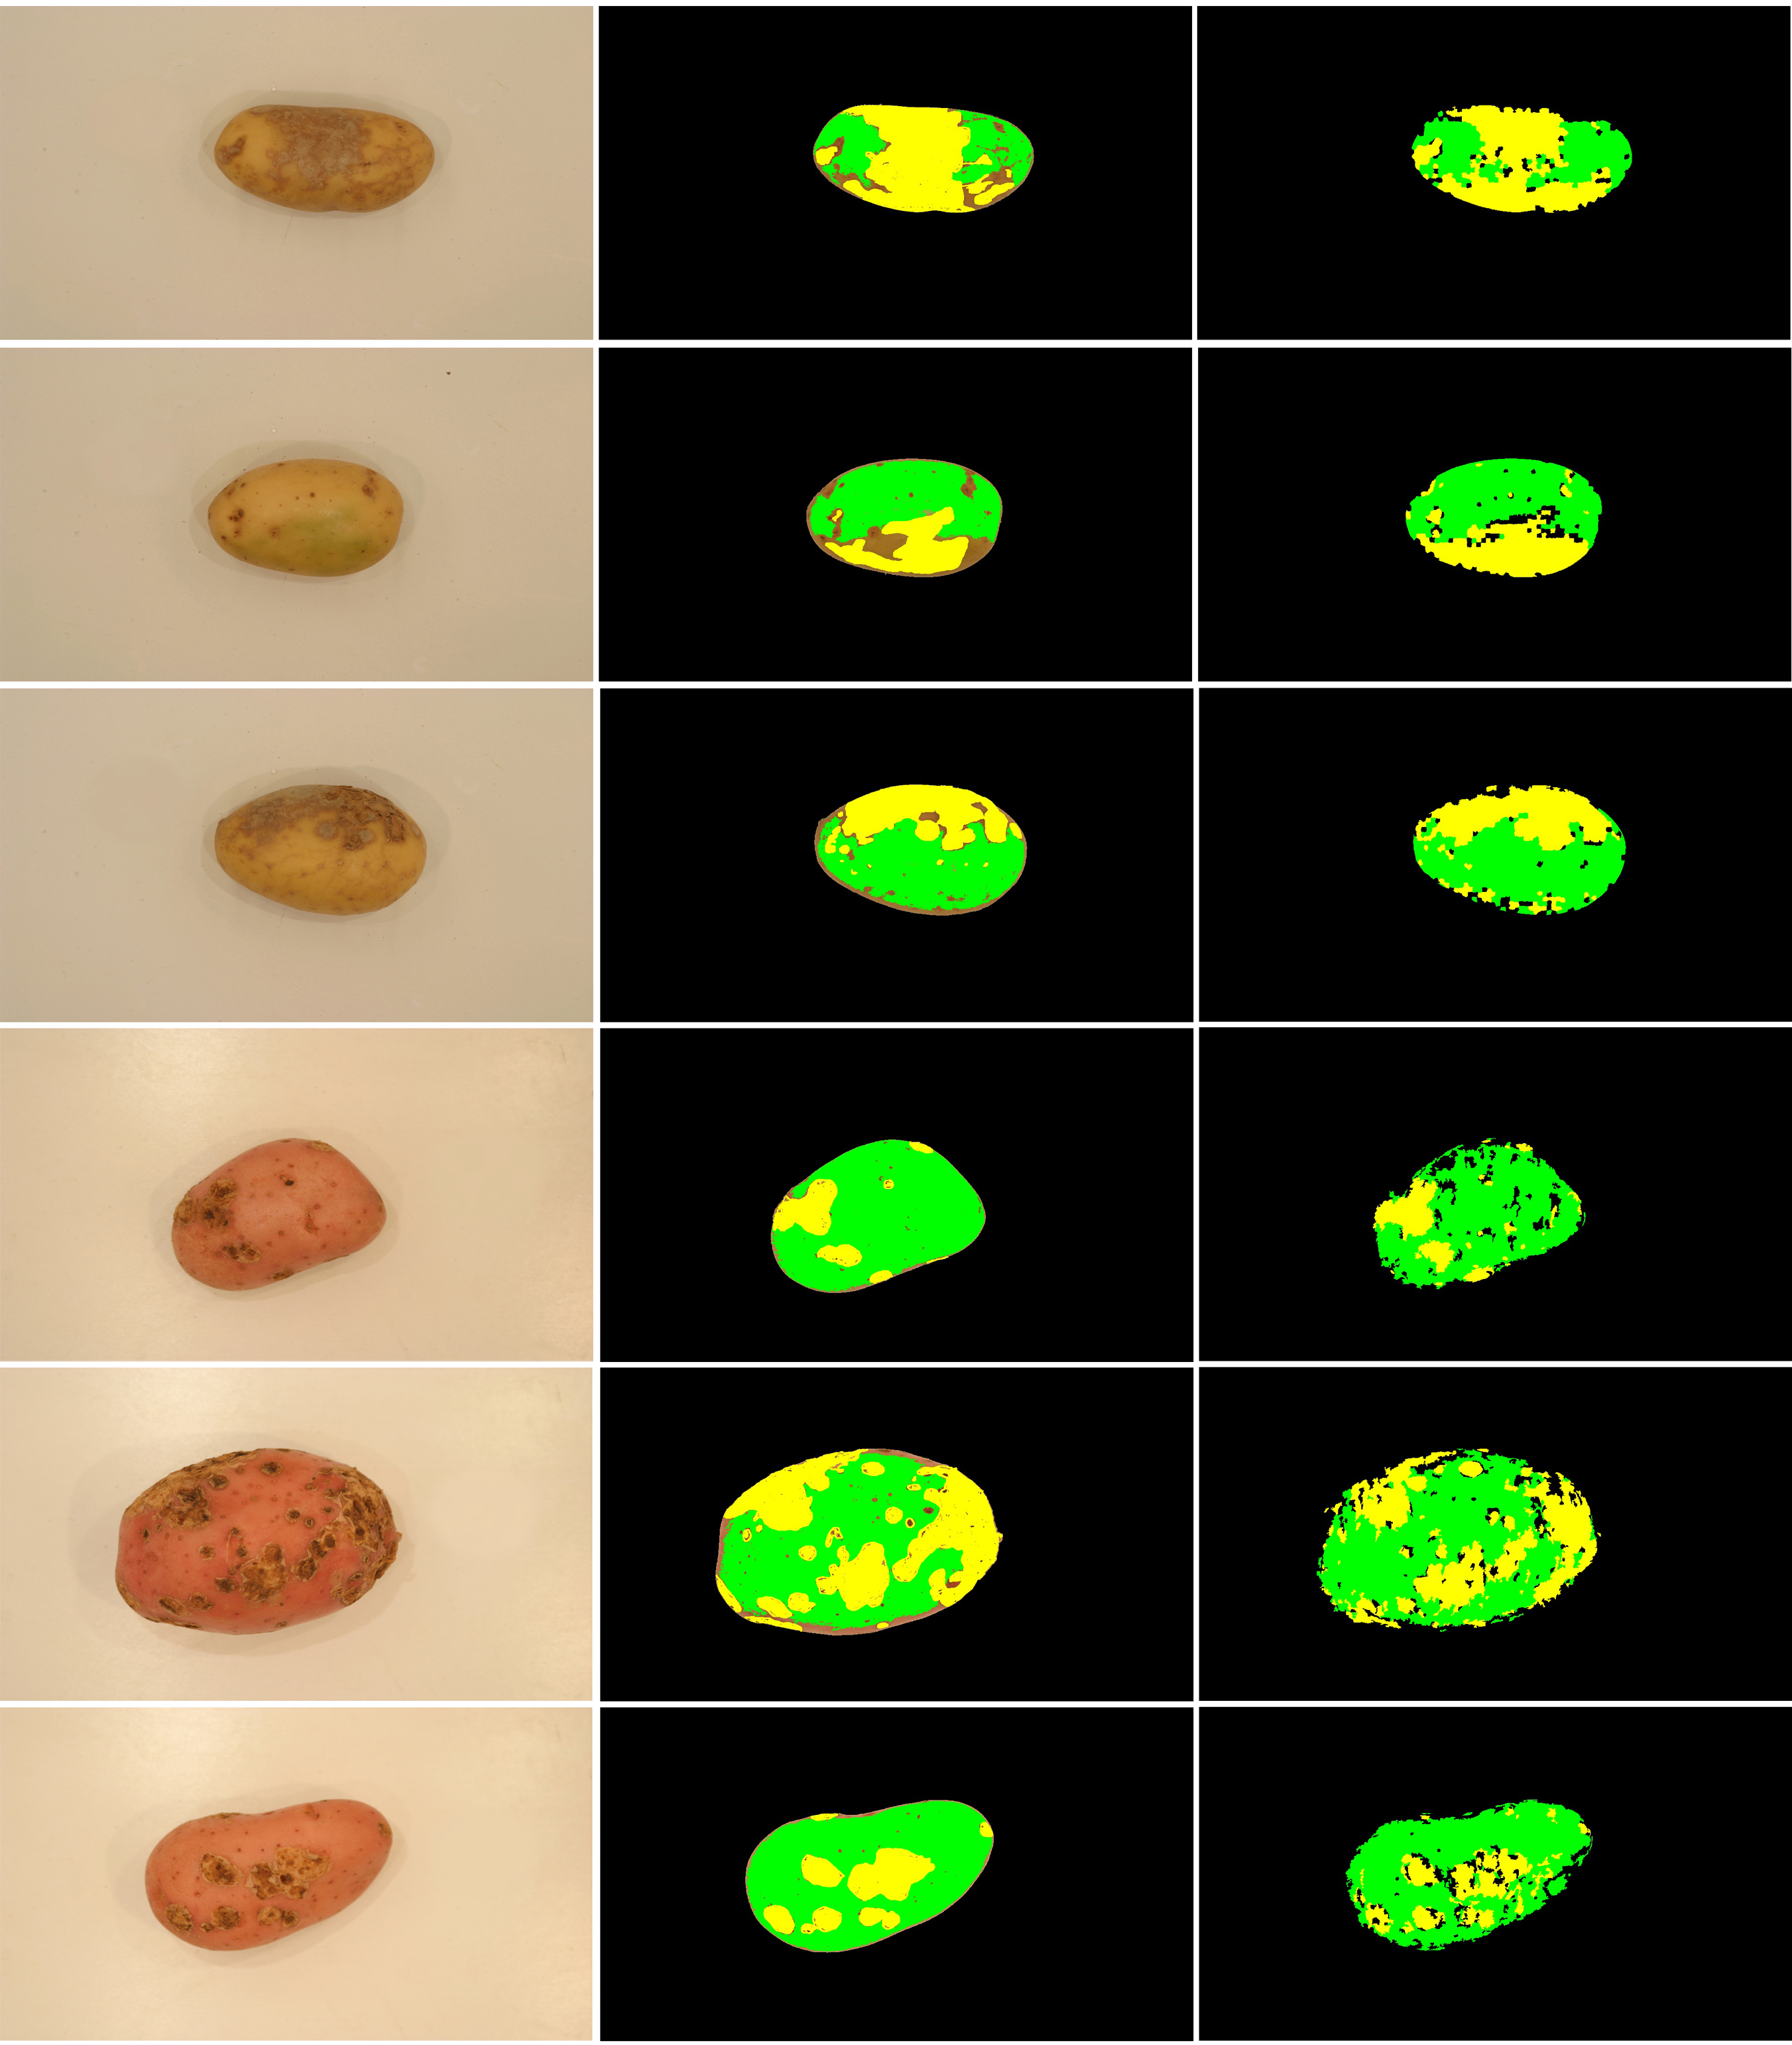
\includegraphics[width=0.8\linewidth]{potatoes.jpg}
\caption{Some of the results produced by the proposed system where we use green and yellow to denote good regions and blemishes respectively. Left column: original images; Middle column: ground truth images; Right column: our results.}
\label{fig:pa}
\end{figure*}

\section{Experimental results and evaluation}
We test the proposed system in two ways. The first one is to evaluate its accuracy for two-label image segmentation. Two-label image segmentation can be used for grading tasks where we partition a potato into blemished and unblemished regions. Then the grading is simply based on the percentage of the size of blemished or unblemished regions. The second one is more complicated. It is designed to evaluate its performance in the tasks of detecting several common potato blemishes through multi-label image segmentation.  

\subsection{Experimental results and evaluation of two-label image segmentation}
In the experiments, two datasets were used. One is a collection of images of 25 white potatoes and the other is that of 41 red potatoes. In each dataset, we only use the ground truth images of 5 potatoes for training. The reason that we only select a small number of images for training is that in real applications, users often tend to label a small number of superpixels in an interactive manner, which requires that the classifier must work well based on a limited amount of training data. 
\begin{figure*} [t]
\centering
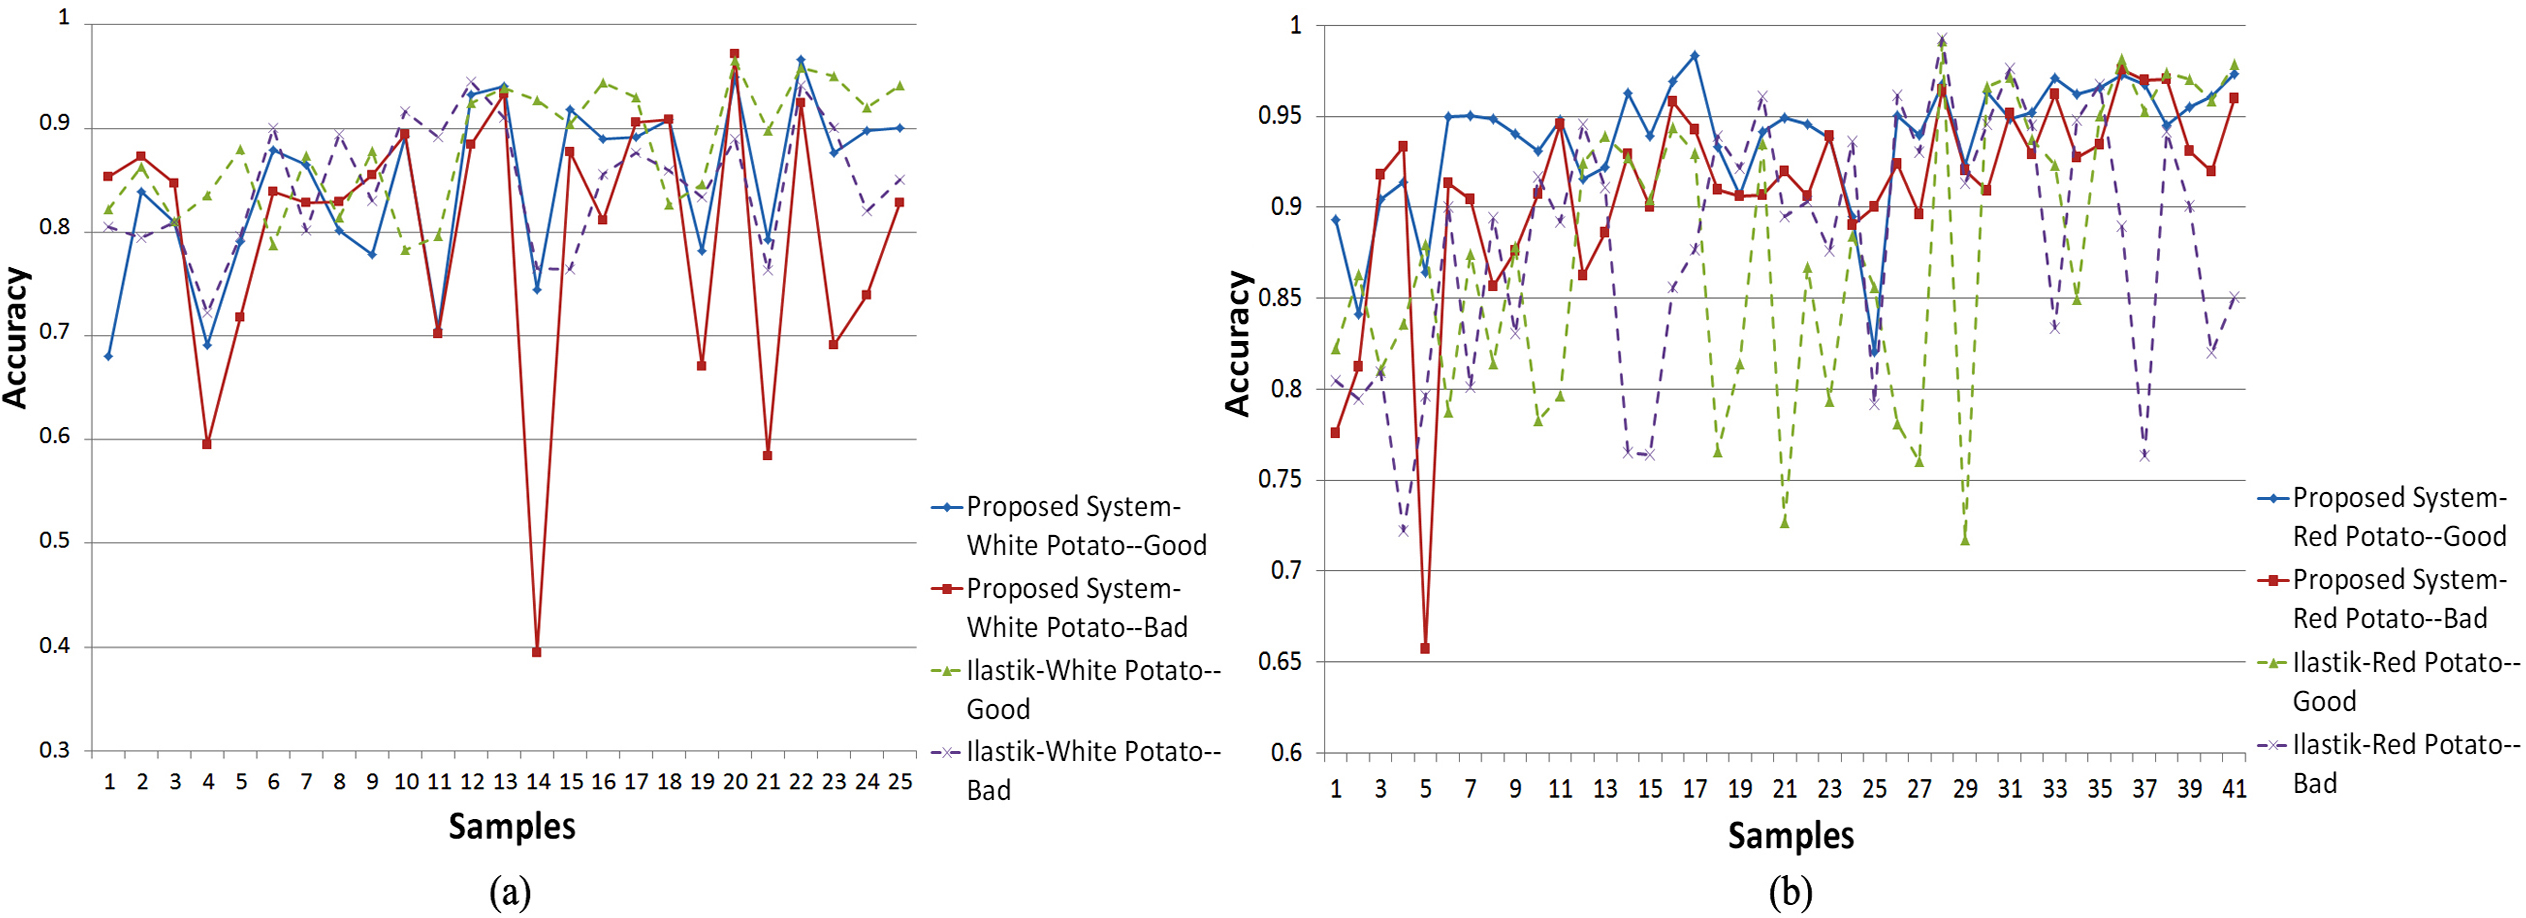
\includegraphics[width=1\linewidth]{ac.jpg}
\caption{Comparative results of two-label image segmentation. (a) Results for 25 white potatoes trained and tested with the proposed system and the system in \cite{SC11}; (b) Results for 41 red potatoes trained and tested with the proposed system and the system in \cite{SC11}}
\label{fig:ac}
\end{figure*}

Some of the results are shown in Fig.~\ref{fig:pa} in association with the corresponding original images and the pixel-wise ground truth images marked by an expert in potato pathology. Note that some areas of high uncertainty or ambiguity were left unmarked, which is inevitable since even under a microscope, the expert could still be unsure about whether a particular region is good or not. These unmarked pixels are ignored during the training of the classifier. Also, our system relies on superpixel-based over-segmentation for the reasons of efficiency and convenient selection of training data. Some holes thus occur, particularly in the regions where the labels change as shown in Fig.~\ref{fig:pa} because one superpixel can be labelled into two different classes equally (they equiprobable classes) so it leads to an unclassified superpixel. One remedy for this is to choose one of the classes randomly. 

To compare the results of the discussed prototype, the state-of-the-art method ilastik \cite{SC11} is used for training and testing with the same potato dataset. The system allows the user to perform segmentation and classification. Users need to mark up locations and provide training data pixel by pixel. This is typically a very tedious task. Classification is based on random forests. This system utilises up to three spatial and one spectral dimension in the feature calculation. It has capabilities like saving classifiers for later batch processing. 

To perform the evaluation, we use the ground truth images of 5 potatoes in each dataset for training. This is actually impossible for the method in \cite{SC11} in practice because human users cannot mark up 5 images with a resolution of $1280 \times 720$ pixel by pixel (but possible for our system based on superpixel which significantly mitigates the manual effort of mark-up). Even so, comparison results of the system in \cite{SC11} to our system is shown in Fig.~\ref{fig:ac}. 

In these figures, we use the following equations to compute the accuracy in detecting the good (blemished) and the bad (unblemished) areas respectively.
\begin{equation}
Acc_{good}=\frac{\left|G_r\cap G_g\right|}{\left|G_r\cup G_g\right|}, \quad Acc_{bad}=\frac{\left|B_r\cap B_g\right|}{\left|B_r\cup B_g\right|}
\end{equation}
where $G_g$ and $B_g$ denote the good and the bad areas (calculated by the number of pixels) in the ground truth images while  $G_r$ and $B_r$ denote the good and the bad areas in the resultant images.
\begin{table*}[t]
\centering
\begin{tabular}{ l||l|l|l|l|l|l }
\hline
   Type&Unblemished & Black Dot& Sliver Scurf& Scab & Greening & Other Blemishes  \\ \hline
   Colour&Green & Blue & White & Cyan & Yellow & Magenta \\
	\hline
\end{tabular}
\caption{The colour code for the visualisation of segmentation results of both white and red potatoes}
\label{tab:t1}
\end{table*}

On average, the accuracy of the system in \cite{SC11} in detecting the good areas for the white potatoes is 0.8807 and for the bad areas is 0.8455, while the average accuracy in detecting the good areas for the red potatoes is 0.8785 and for the bad areas is 0.8801. In comparison, the average accuracy of our system in detecting the good areas for the white potatoes is 0.8451 and for the bad areas it is 0.7983, while the average accuracy in detecting good areas for the red potatoes is 0.9372 and for the bad areas it is 0.9099. It can be seen that in terms of accuracy, our system is comparable with the state-of-the-art method. The results of the prototype system introduced in this paper, especially in detecting bad areas, can be improved by using some other features like frequency domain features. However, the prototype system provides a trade-off between accuracy and speed that makes it suitable for training in quality control tasks. Also, note that our method is based on labelling superpixel regions while in one superpixel there could be different types of potato regions (good or bad) but the competing method is pixel-wise. When we use the ground truth images of 5 potatoes to train our system, we always need to first convert the pixel-wise ground truth images into superpixel-wise ones. Such a conversion inevitably introduces errors. Furthermore, it is worth pointing out that in order to facilitate the evaluation, all of the experiments were implemented based on a `one-off' operation, which means that we actually disable the powerful function of the system that allows the user to modify the training data interactively. In general, the segmentation output by our method can be easily improved by interactively modifying the training data. This can be demonstrated by our video on YouTube.
\begin{figure*} [htbp!]
\centering
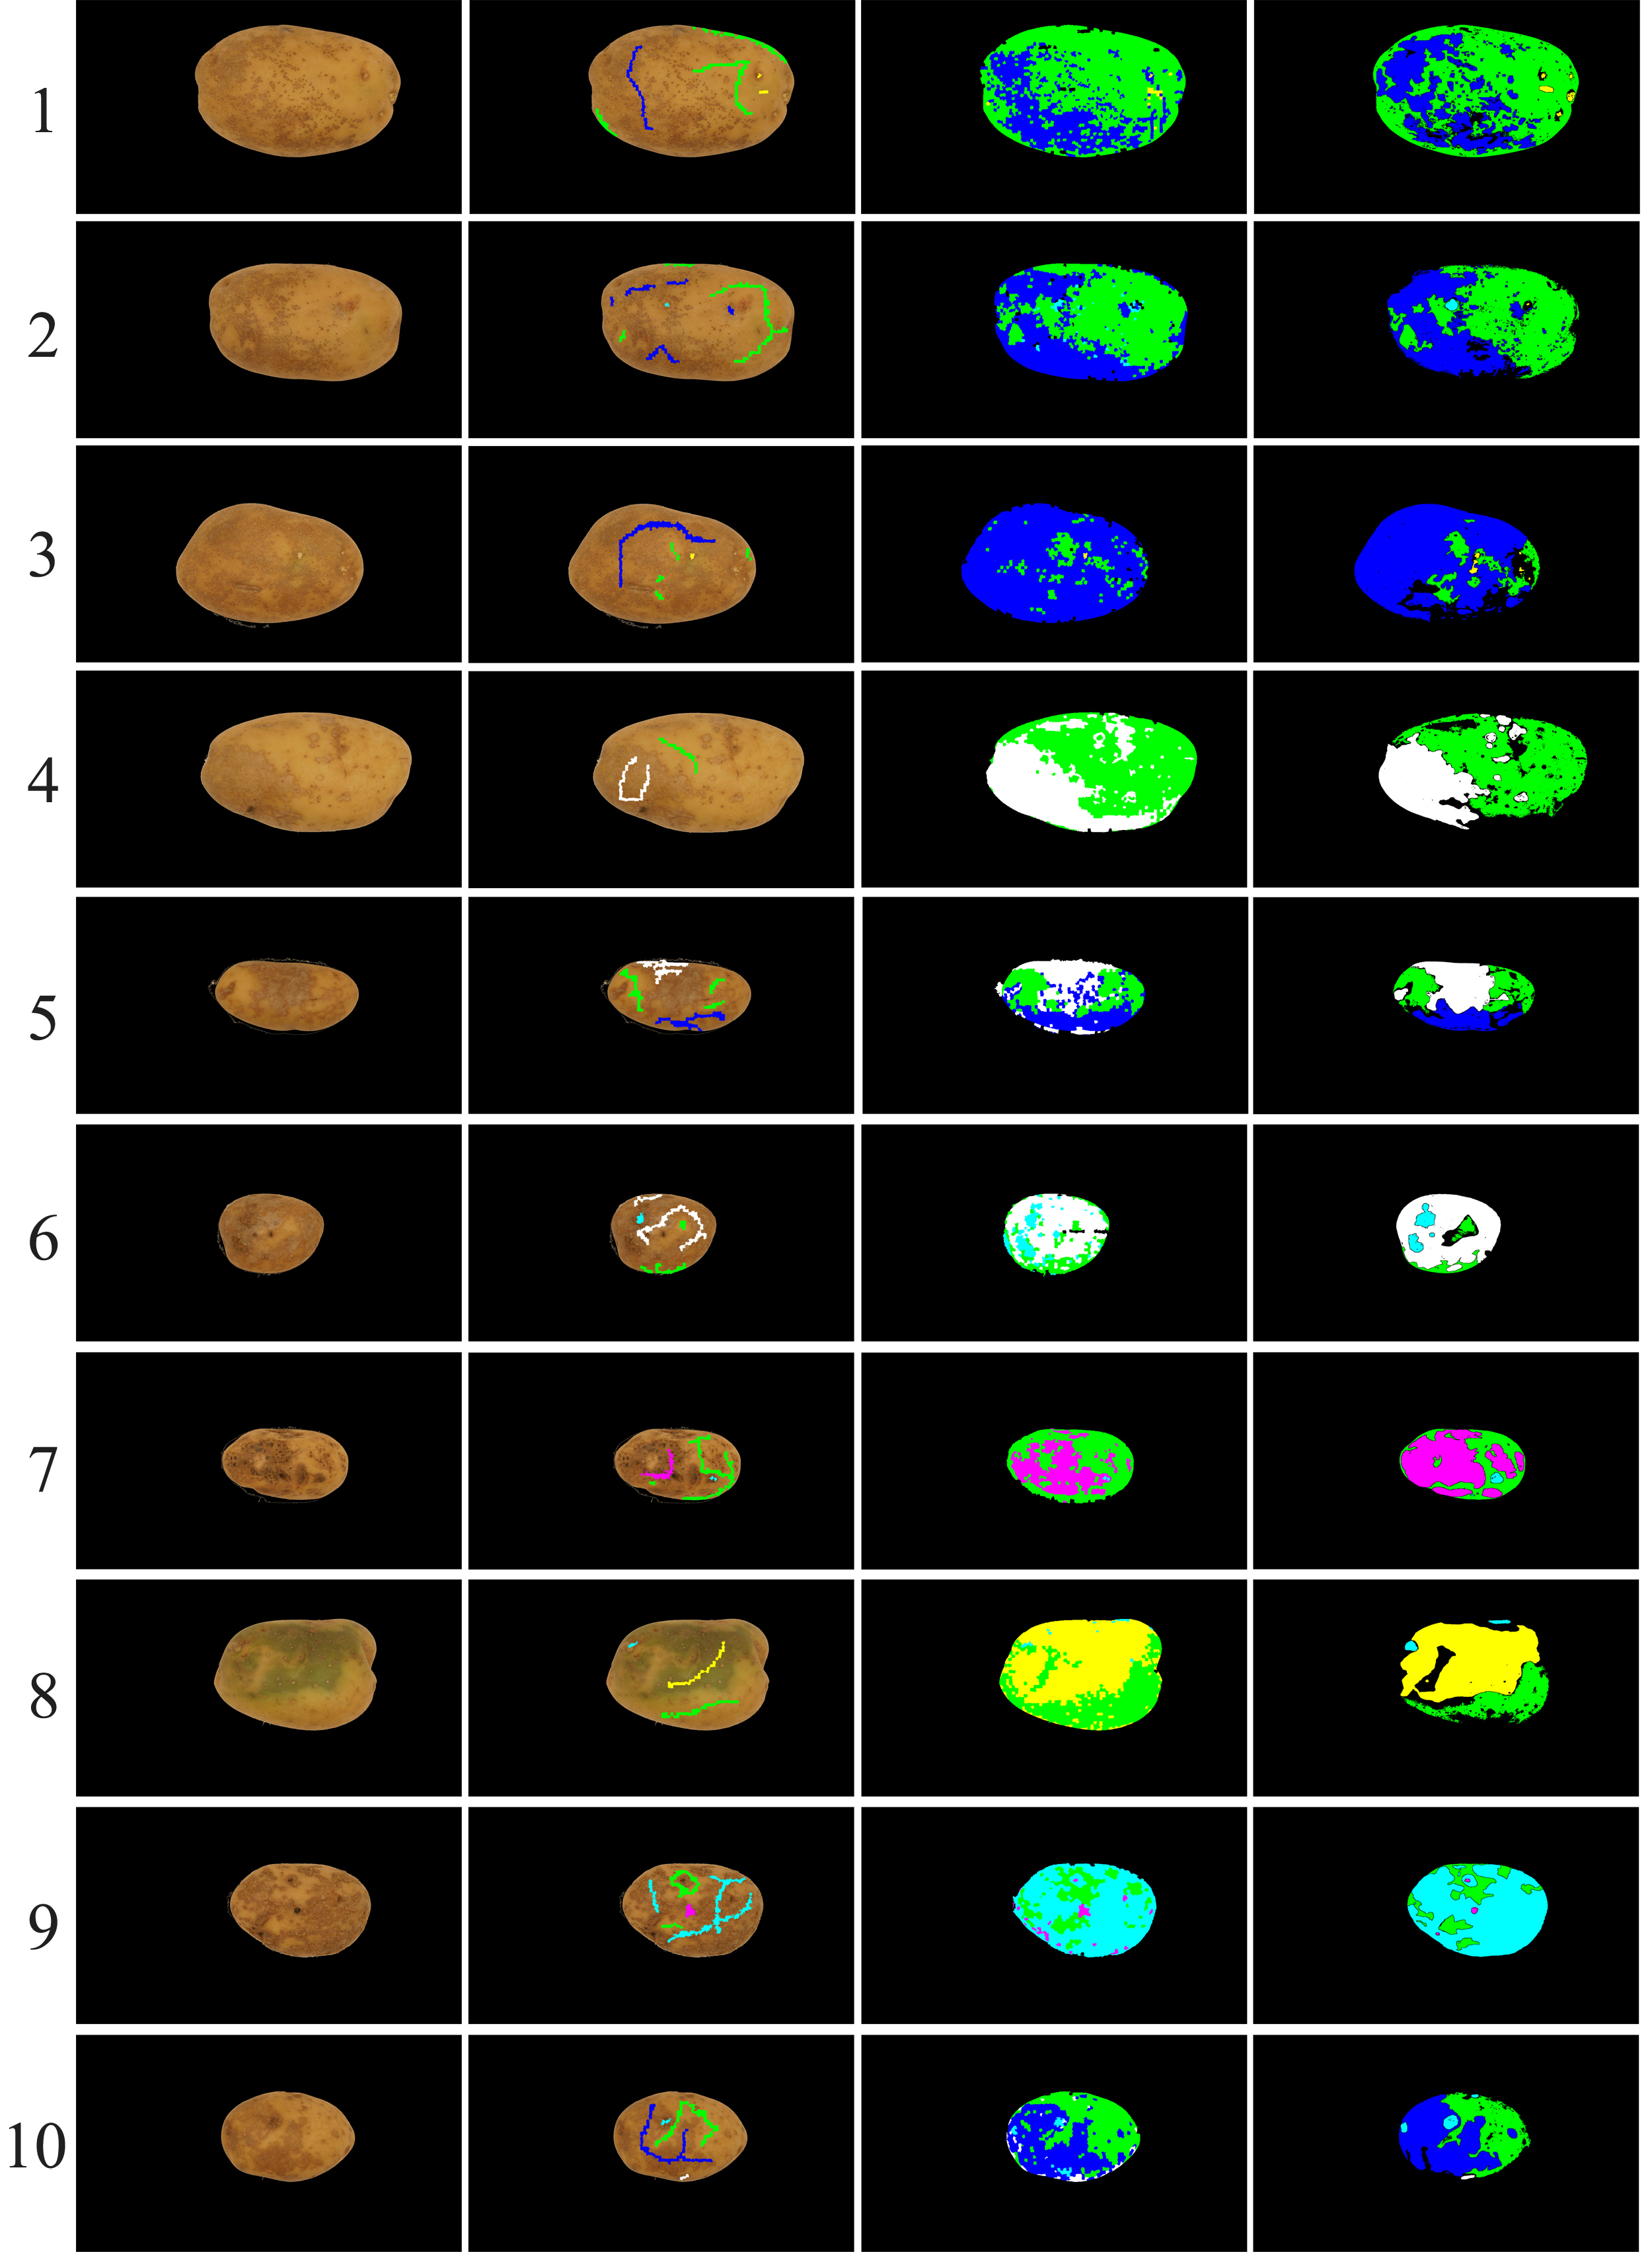
\includegraphics[width=0.95\linewidth]{r1.jpg}
\caption{Segmentation results of 10 images of white potatoes. From left to right: Original images, training data, Segmentation results, ground truth images}
\label{fig:r1}
\end{figure*}

\subsection{Experimental results and evaluation of multi-label image segmentation}
We also tested our system using 102 images of white potatoes and 41 images of red potatoes containing different types of blemishes. The results of 10 white potatoes are shown in Fig.~\ref{fig:r1}. In Fig.~\ref{fig:r1}, we use different colours to represent different types of potato blemishes. The colour code of this multi-label image segmentation is shown in Table~\ref{tab:t1}. It can be observed that our system just utilises a tiny amount of training data, typically several brush strokes composed of a couple of superpixels and output segmentations visually analogous to the corresponding ground truth images.

Based on the ground truth data, we managed to compute the confusion matrices for quantitatively evaluating the performance of our system. Fig.~\ref{fig:r2} shows the confusion matrices corresponding to the 10 white potatoes shown in Fig.~\ref{fig:r1}.

For Potatoes 1 and 3, according to the confusion matrices shown in Fig.~\ref{fig:r2}, the classification results for black dot and healthy areas are very good despite the fact that black dot is a type of blemish that can cover several pixels not a whole super-pixel.

For Potato 2, it can be seen that the results for scab and greening  are not good. The reason is that the region of greening is so tiny to be put in one or two superpixel(s) and it is hard to part it for traing and testing. In other words,  training data for greening is noisy. On the other hand,  the colour information for the scab region contains  some information from neighbouring black dot region (for superpixel algorithm it is very hard to segment these close neighbours) and that affects both training and testing. Overall, classification accuracy for unblemished area and black dot is so high that makes this system reliable in quality control tasks.

The segmentation result of Potato 4 demonstrates that the system is capable of distinguishing between silver scurf and healthy regions. This is due to the fact that our feature extraction  covers colour information  to recognise these areas.
\begin{figure*} [htbp!]
\centering
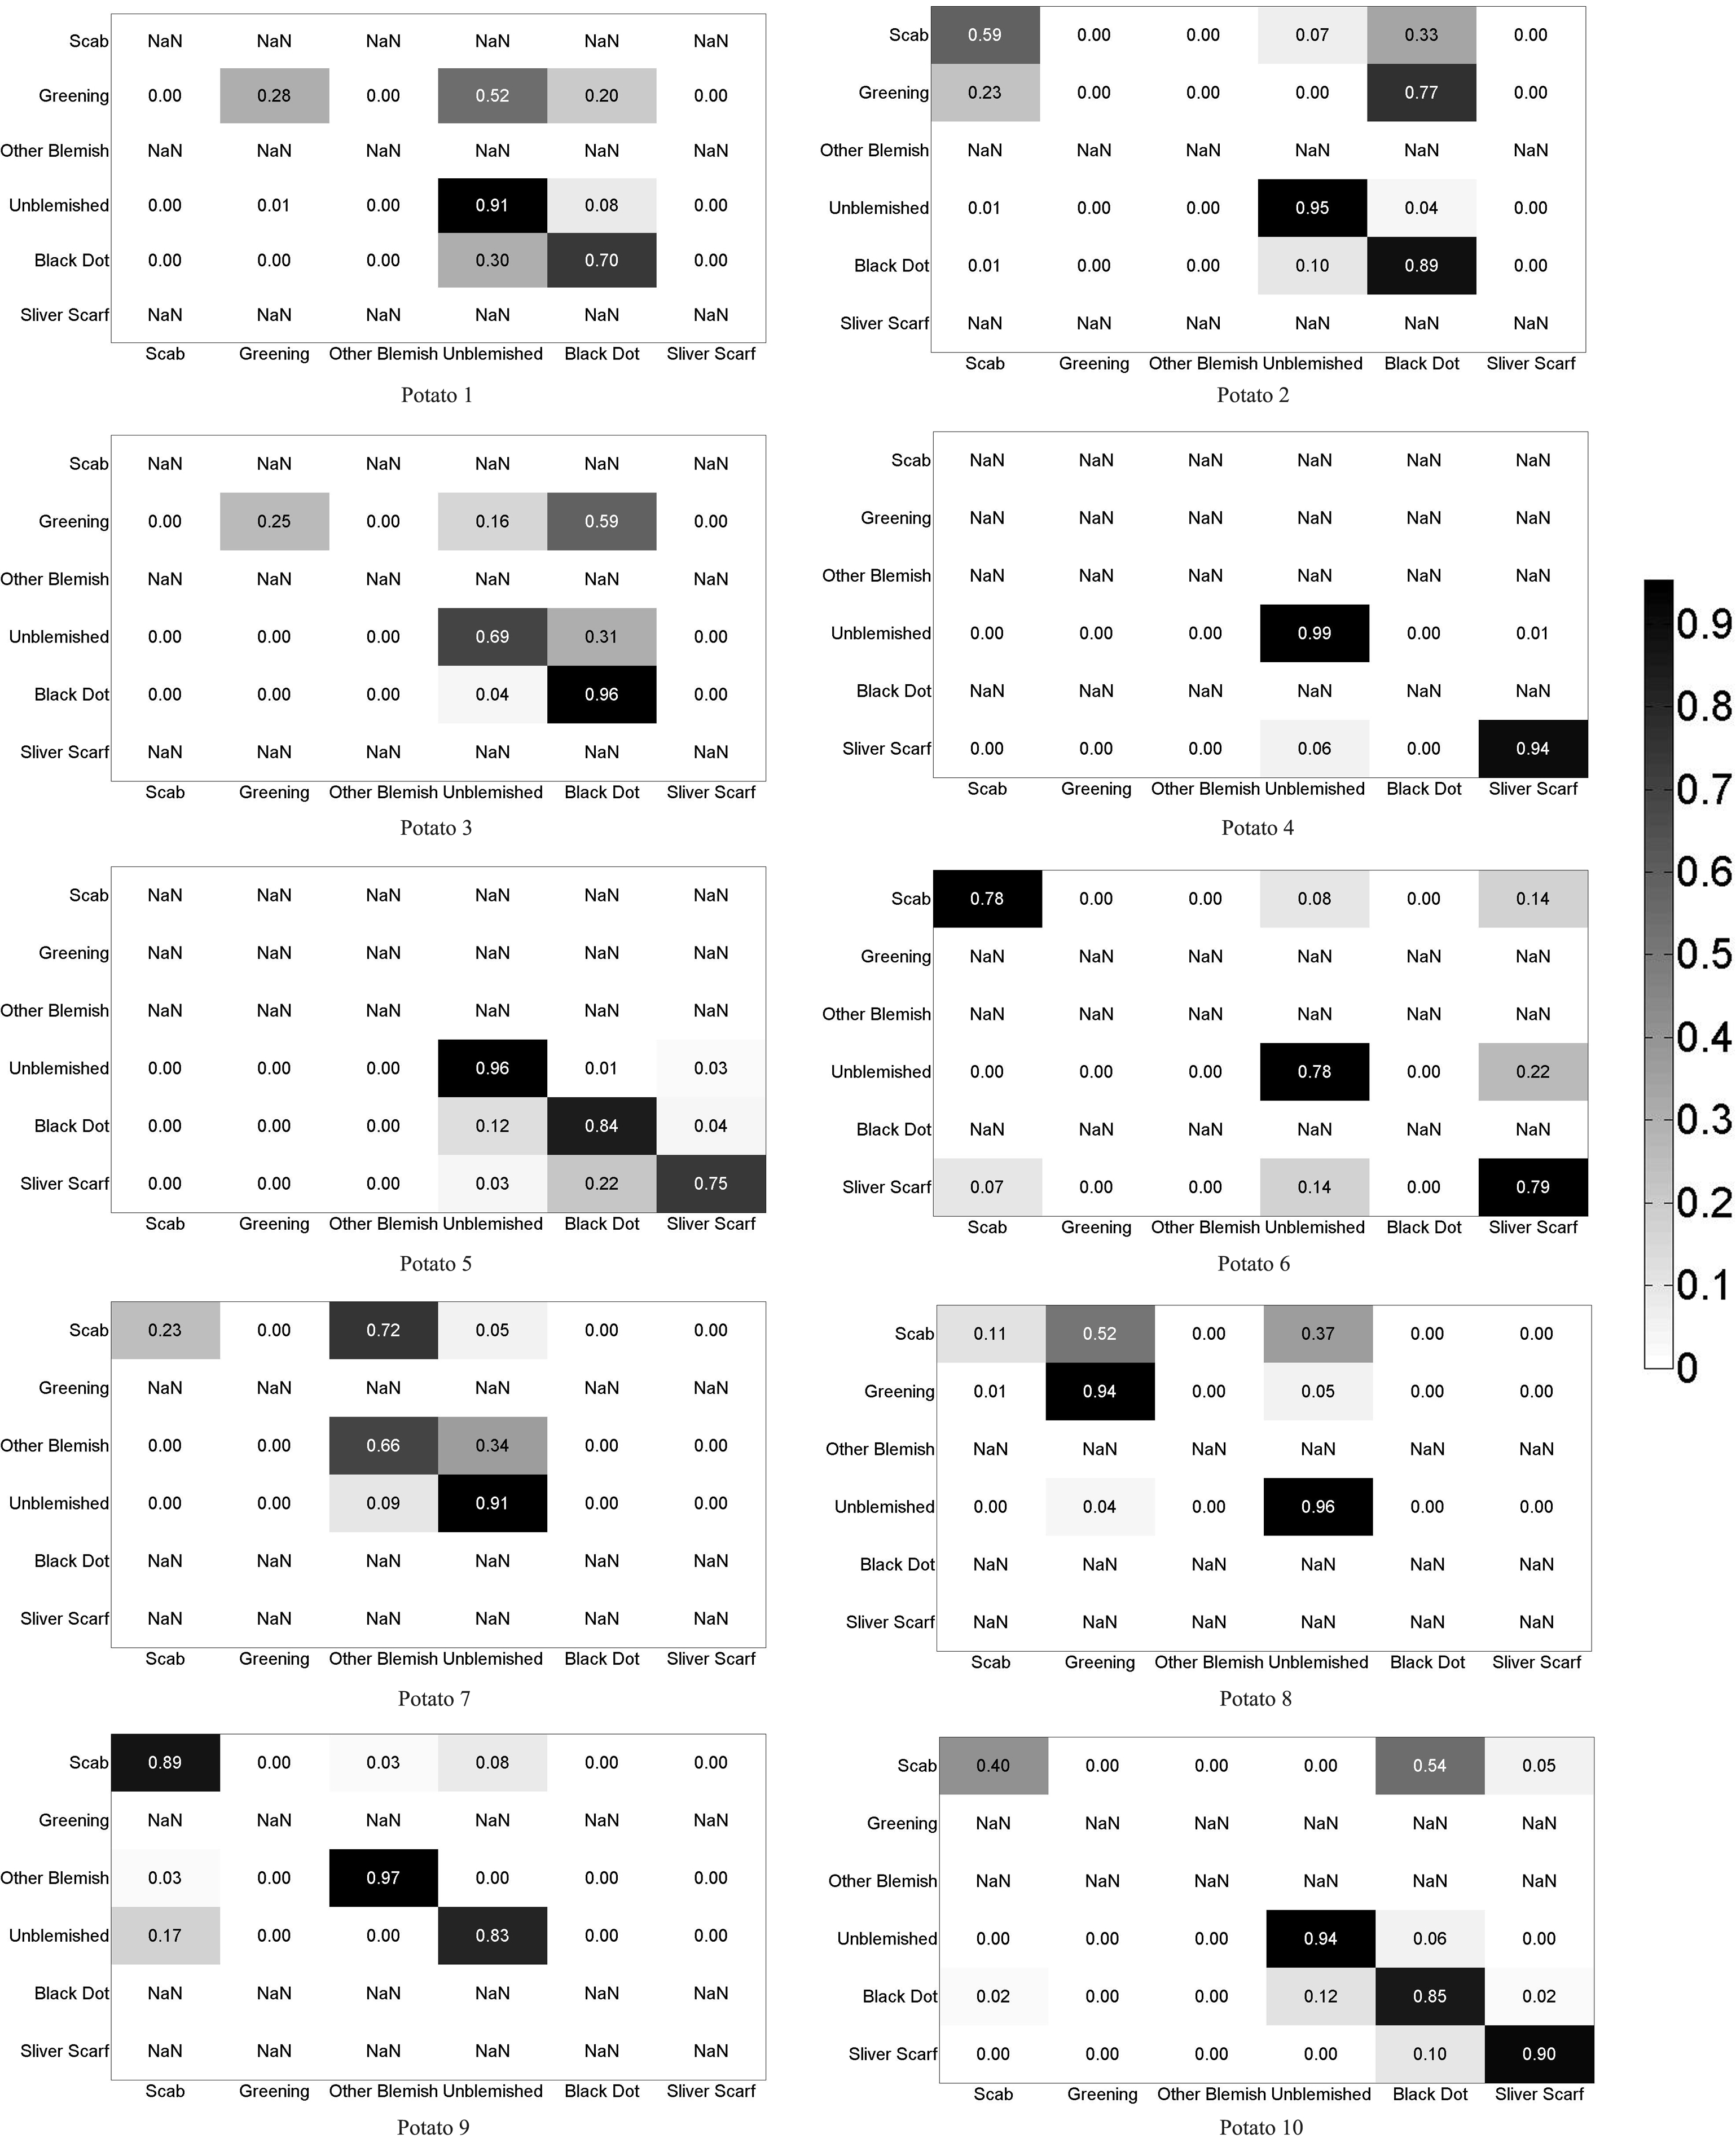
\includegraphics[width=1\linewidth]{r2.jpg}
\caption{Confusion matrices of the segmentation results of 10 white potatoes where `NaN' denotes that there is no such type of blemish in the image.}
\label{fig:r2}
\end{figure*}
\begin{figure*} [t]
\centering
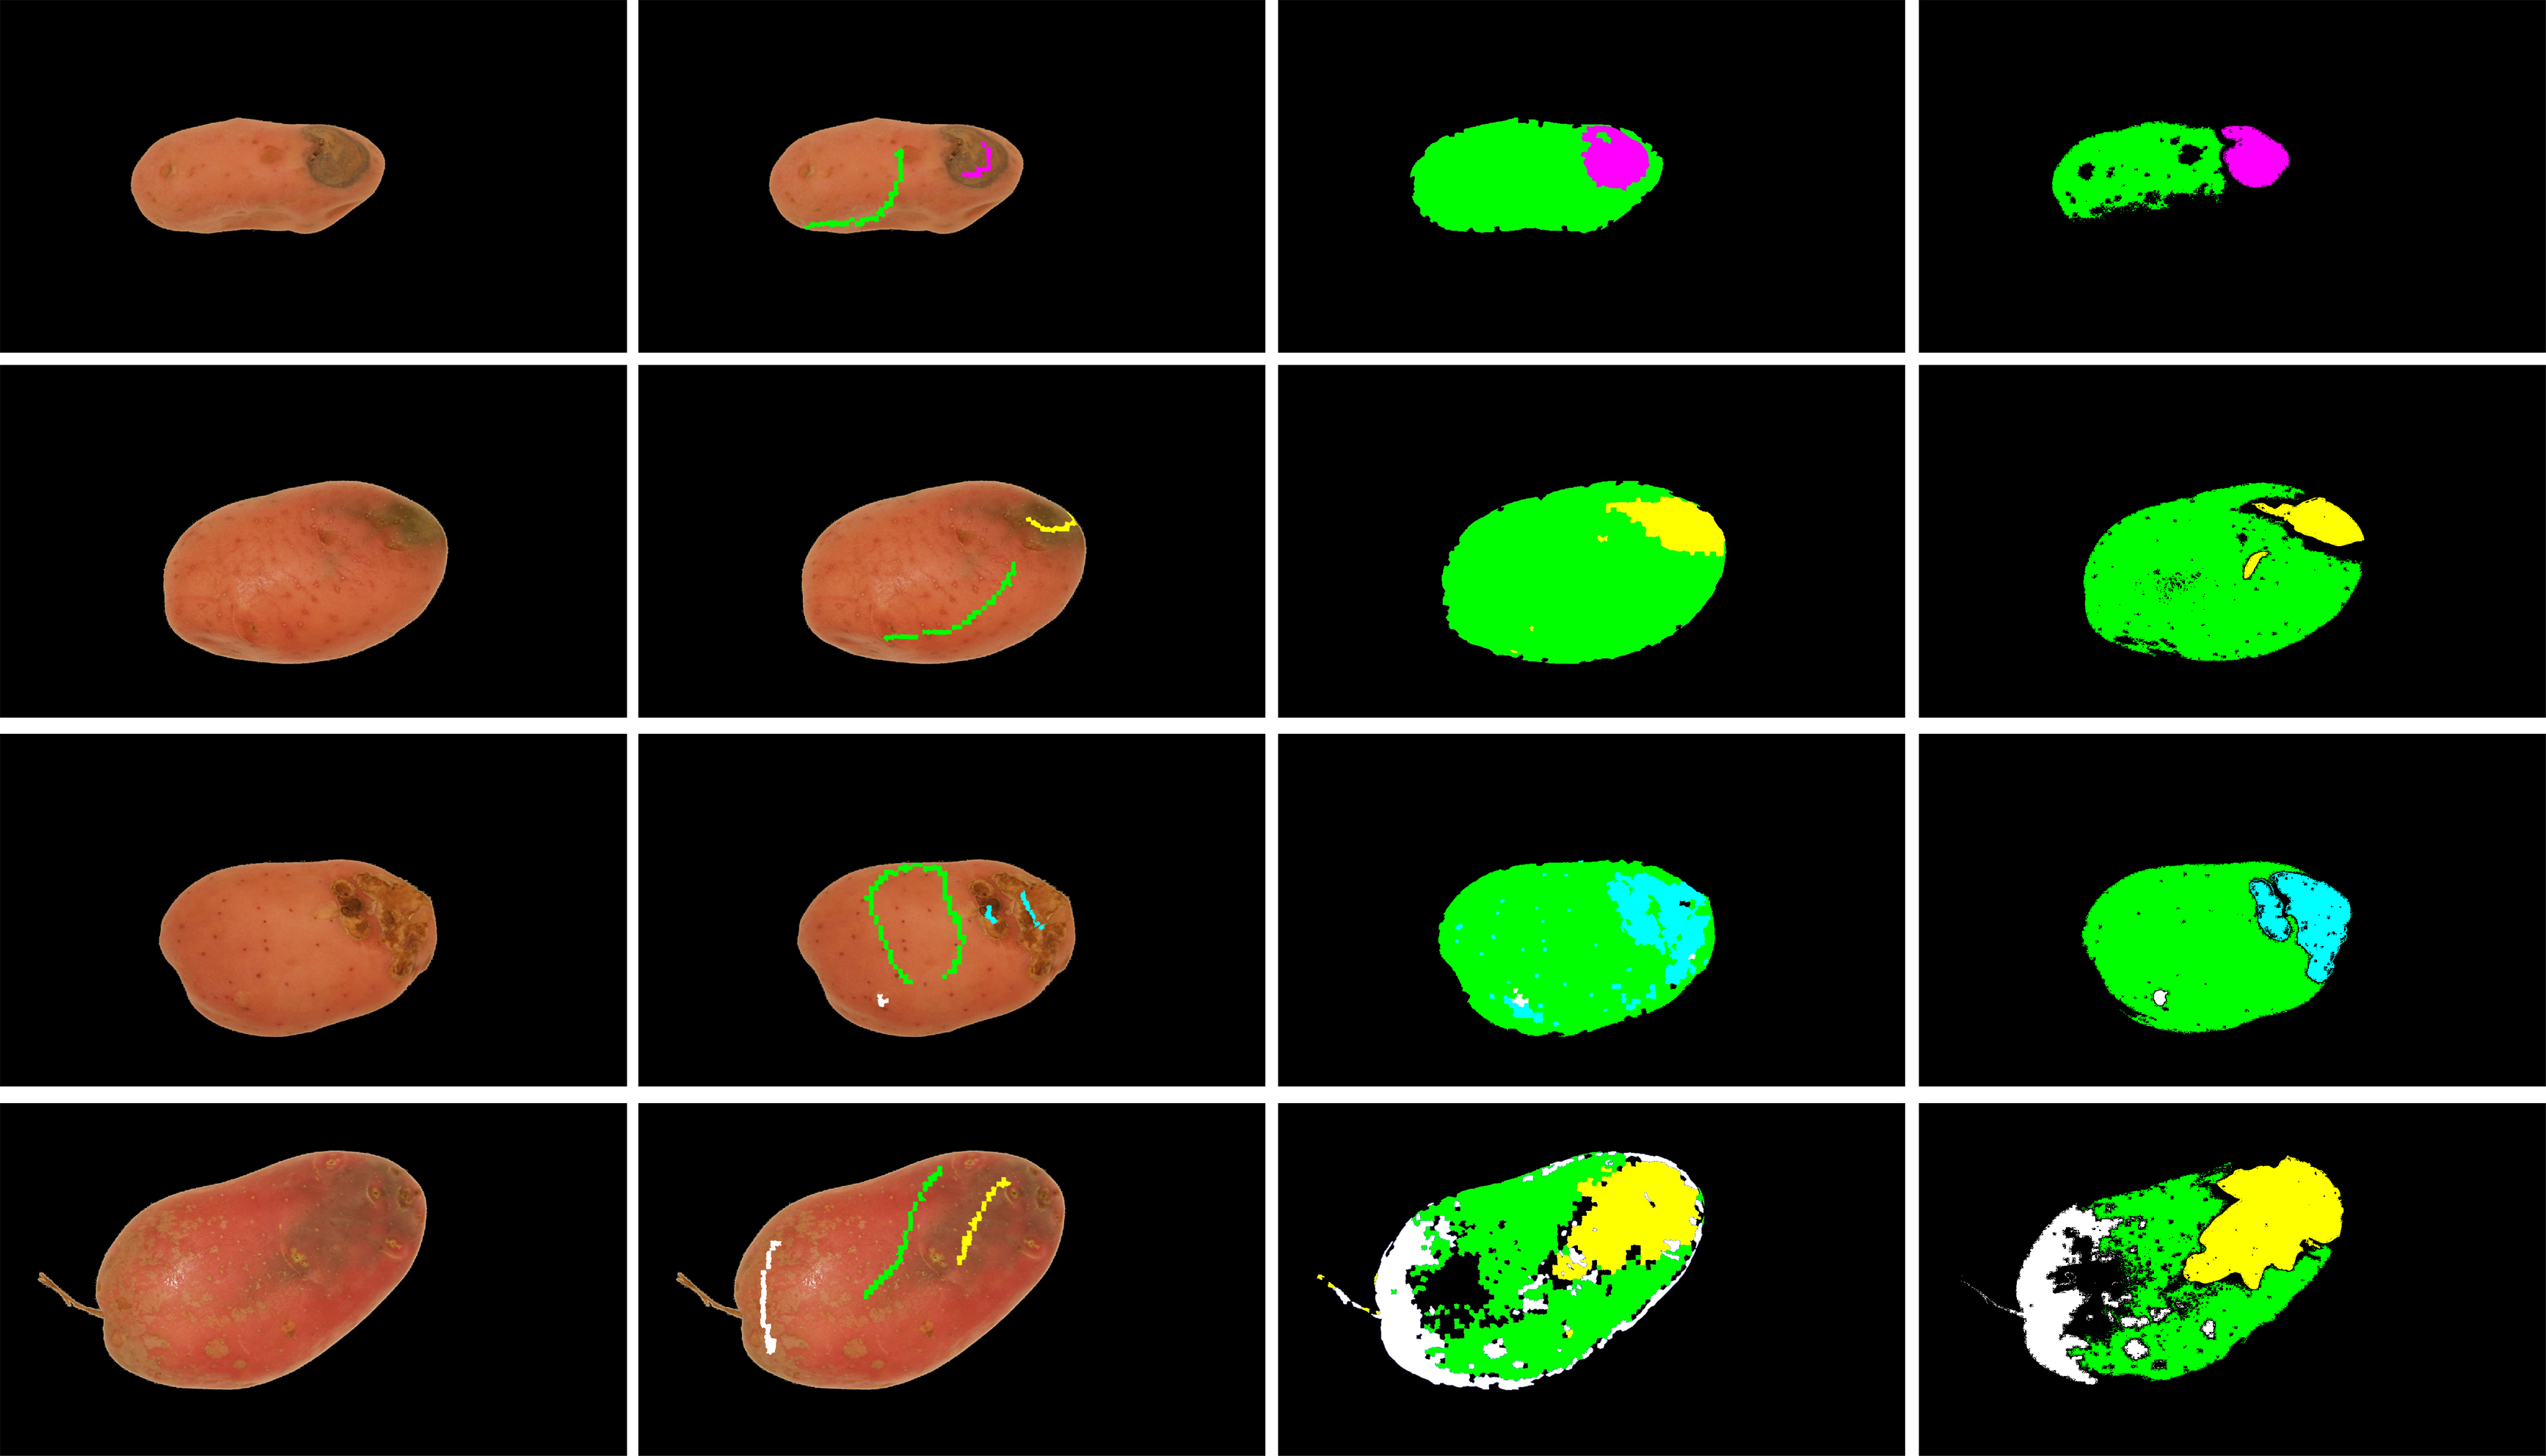
\includegraphics[width=1\linewidth]{r3.jpg}
\caption{Segmentation results of 4 images of red potatoes. From left to right: Original images, training data, Segmentation results, ground truth images}
\label{fig:r3}
\end{figure*}

The segmentation results for Potatoes 5 and 6 are very good. In the image of Potato 5, we have three classes which two of them are very hard to tell apart: black dot and silver scurf. For Potato 6, it can be seen that our system can distinguish scab and silver scurf reliably. The visual difference between scab and silver scurf is a key to have  much less noisy data while training hence leading to a good segmentation.

Potato 7 contains three classes: unblemished area, scab and other blemish type. Colour information of other blemish type is similar to scab which makes it hard to distinguish. But, both blemish types are very different to the unblemished area by variations in colour information.

For Potato 8, the performance to distinguish between unblemished area and greening area is very good. But scattered scab regions are so tiny to be put in one or two whole superpixels. This makes training noisy.

As a comparison to Potato 7, Potato 9 contains the same three blemish types. But since here the colour of other blemish type is quite different from that of the scab, the system outputs a highly accurate segmentation result.  

Potato 10 contains three blemishes: scab, black dot and silver scurf. According to the confusion matrix, the only downside is to detect scab region as they are mostly misclassified as black dot. Again this is due to the fact that superpixels can cover both regions in neighbouring parts which makes us a noisy training data. 

\begin{figure*} [t]
\centering
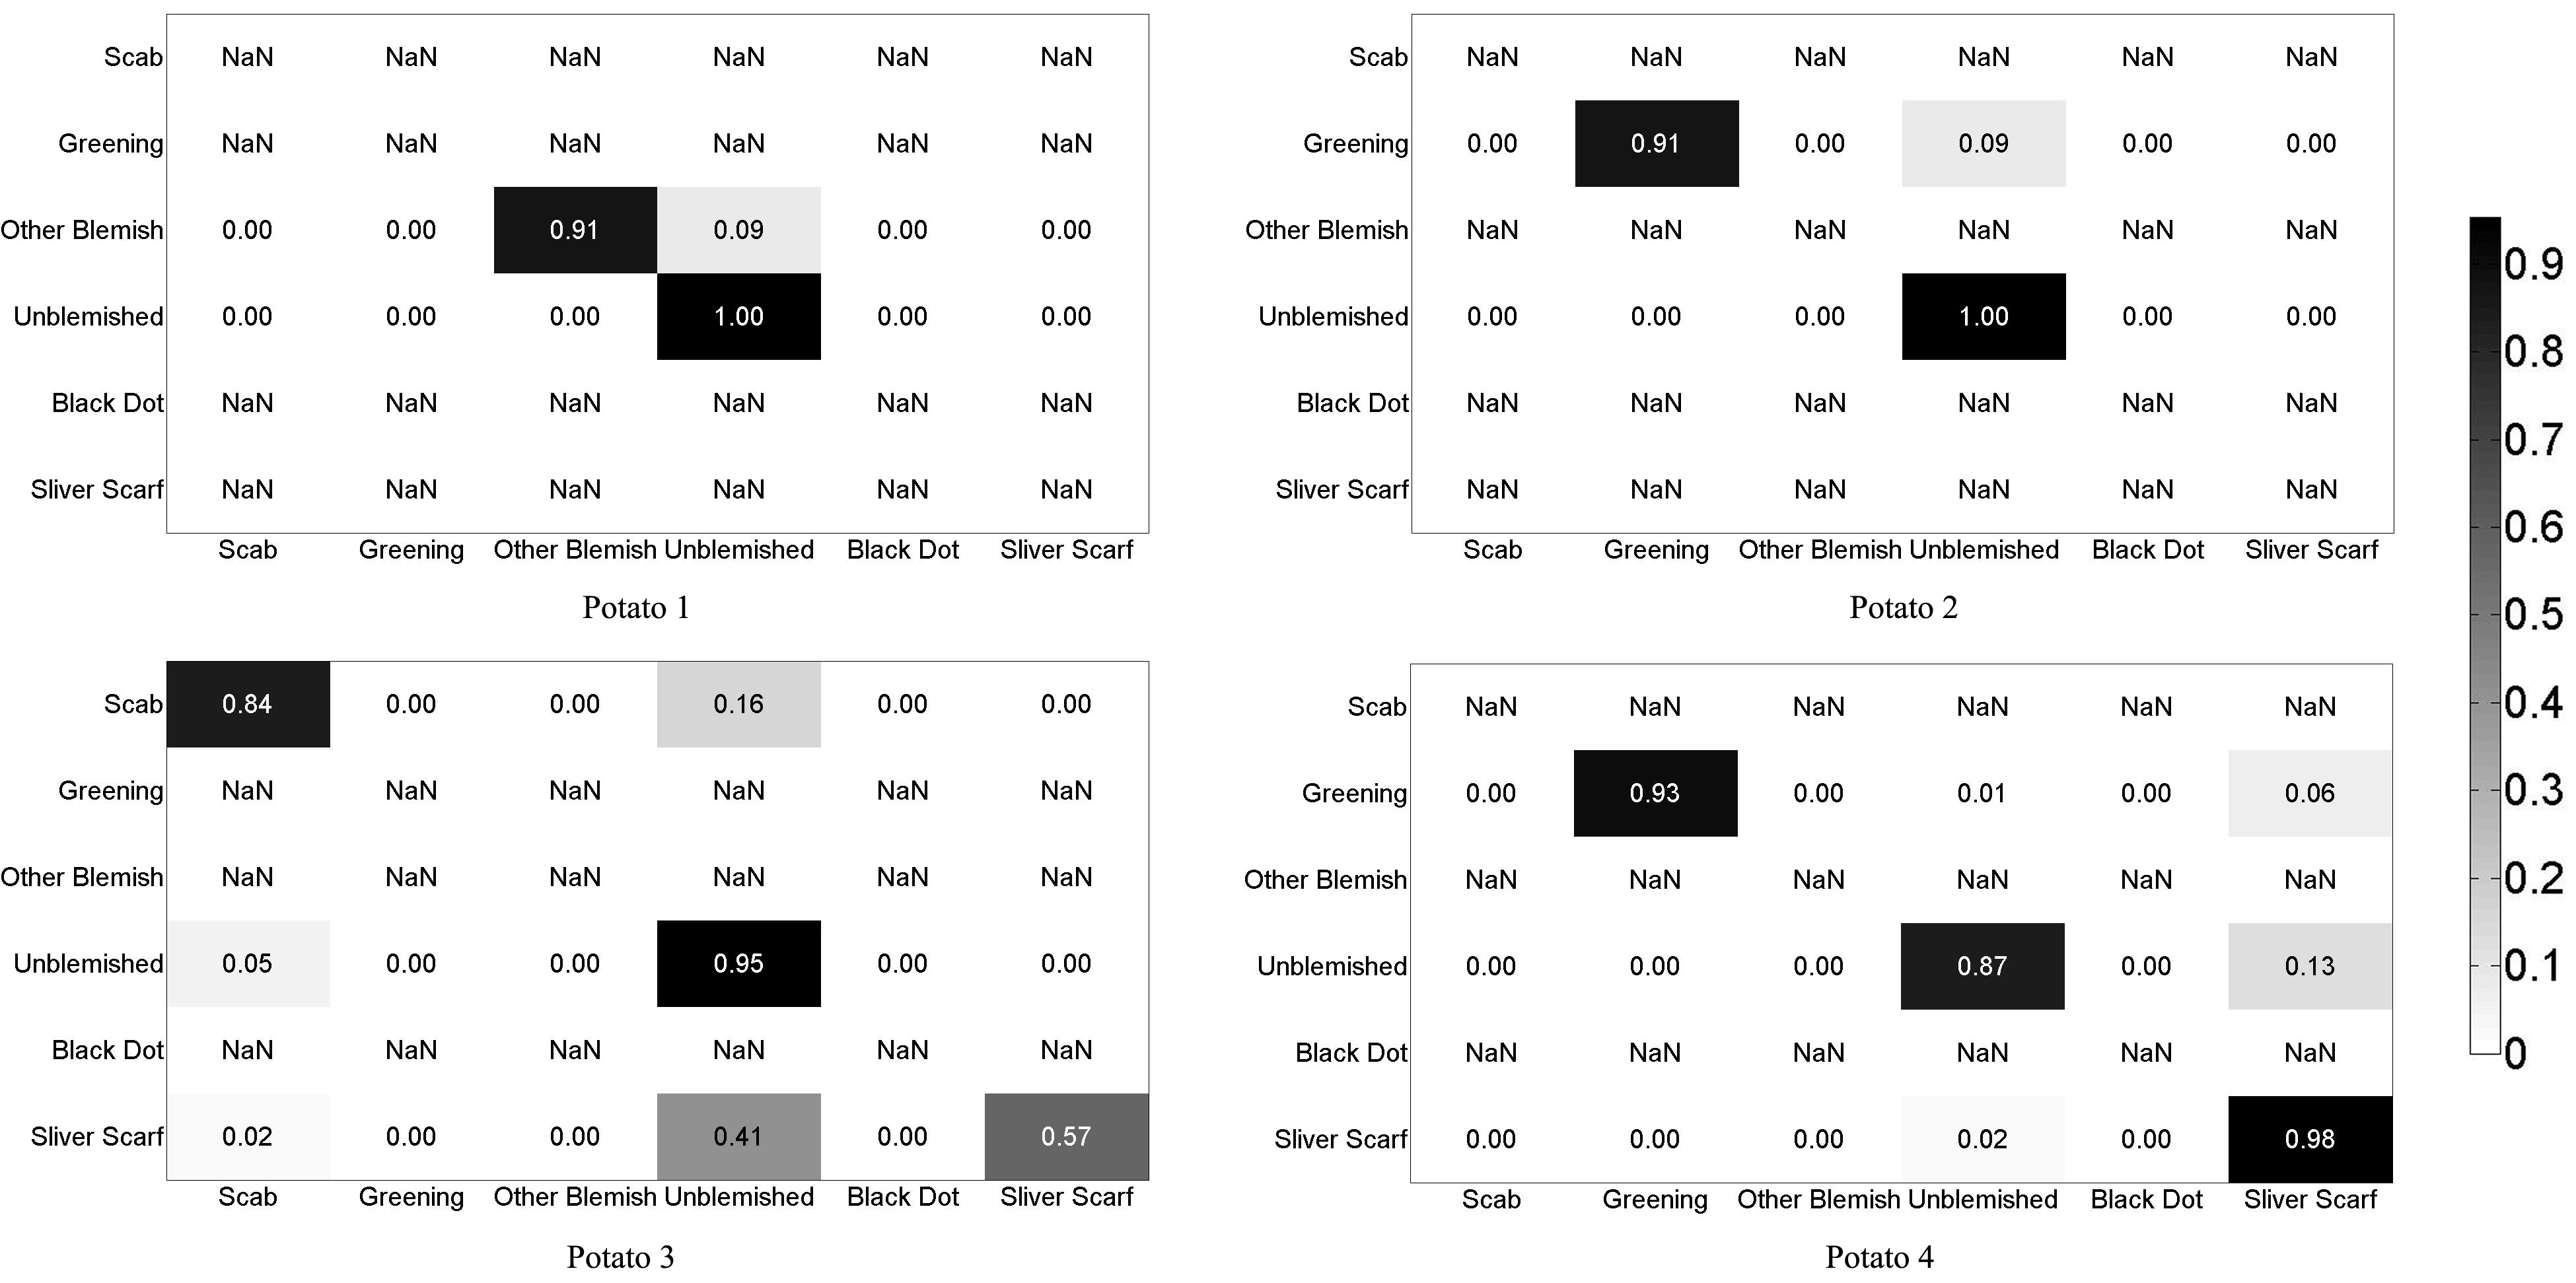
\includegraphics[width=1\linewidth]{r4.jpg}
\caption{Confusion matrices of the segmentation results of 4 red potatoes where `NaN' denotes that there is no such type of blemish in the image.}
\label{fig:r4}
\end{figure*}

Figs~\ref{fig:r3} and \ref{fig:r4} show some of the results of the red potatoes. It can be seen that the performance of our system on the red potatoes are even better. This is mainly because the colour variation in the red potato images are generally larger than that in the white potatoes. In general, the experiments using both white and red potatoes demonstrate that the proposed system is quite effective to detect potato blemishes (or the defects of other types of foods such as fruits and beans) as long as the user can give correct training data in the interaction. Sometimes, even if the training data are slightly wrong or corrupted by noise, the system is still capable of producing good results.

\subsection{Speed}
Obviously the speed of the proposed system will vary, mainly depending on how many training data the user selects. And usually, the more selected training data, the more accurate the classification results. We thus demonstrate that our system can be implemented in real-time through our demonstration video on YouTube. The video recorded typical operations of the system using a PC with a dual core 2.13GHz CPU, 4GB RAM and a GeForce GTX 570 graphics card. It can be seen that the run time for classifying one image is usually 1 or 2 seconds, sometimes even less than 1 second.

\section{Conclusions}
The presented system based on interactive image segmentation shows that a human-in-the-loop scheme is crucial to deliver an effective and efficient solution to the real application of potato blemish detection. With the help of human expertise, a tiny amount of, but highly informative and discriminative training data are provided in an interactive manner. In comparison, traditional offline training requires a large amount of data, which inevitably slows down the processing but does not necessarily improve the segmentation results due to the redundancy within the training data. The experimental results also demonstrated that the introduction of superpixels for over-segmentation does not deteriorate the classification significantly but it accelerates the classification a lot.

There are several possible improvements to the image segmentation method used in our system. First, a pixel-wise refinement might be needed to further improve the accuracy of the classification. In particular, notably in Fig.~\ref{fig:pa} and Fig.~\ref{fig:r1}, a number of disagreements between ground truth and classification results were located around the boundaries of ground truth blemishes. Albeit occasionally, some superpixels straddle two types of regions. In these cases, such superpixels have to be further segmented into the pixel level. Second, while the features are considered in the current classification are all texture features, the involvement of other types of features such as shape features could help to more accurately classify some specific potato blemishes which are distinctive mainly in terms of shape. Thirdly, the proposed system which estimates potato blemishes relies only on 2D information, while a real world scenario we would have to consider the entire surface area of a 3D tuber. 3D information is especially useful in the accurate computation of the areas of the blemishes for grading purpose since currently we actually compute the area of the 2D projection of a blemish region. This will cause errors, particularly in the boundary region of the potato shown in a 2D image. By conducting future research aiming at these 3 improvements, we hope that we can further develop a more powerful and reliable system for real applications.
% For tables use


\begin{acknowledgements}
This work is supported by Technology Strategy Board. This support is gratefully acknowledged. Many thanks to Nigel Allinson and Chris Waltham for the design and build of the image capture set-up shown in Fig.~\ref{fig:pro}. We also thank Graeme Stroud from Potato Council for preparing the ground truth images.
%If you'd like to thank anyone, place your comments here
%and remove the percent signs.
\end{acknowledgements}

% BibTeX users please use one of
%\bibliographystyle{spbasic}      % basic style, author-year citations
\bibliographystyle{spmpsci}      % mathematics and physical sciences
%\bibliographystyle{spphys}       % APS-like style for physics
\bibliography{ref}   % name your BibTeX data base
\end{document}
% end of file template.tex

